% !TEX root = thesis.tex

% Front cover
% \includepdf{cover-front.pdf}

% Half-title
\maketitle


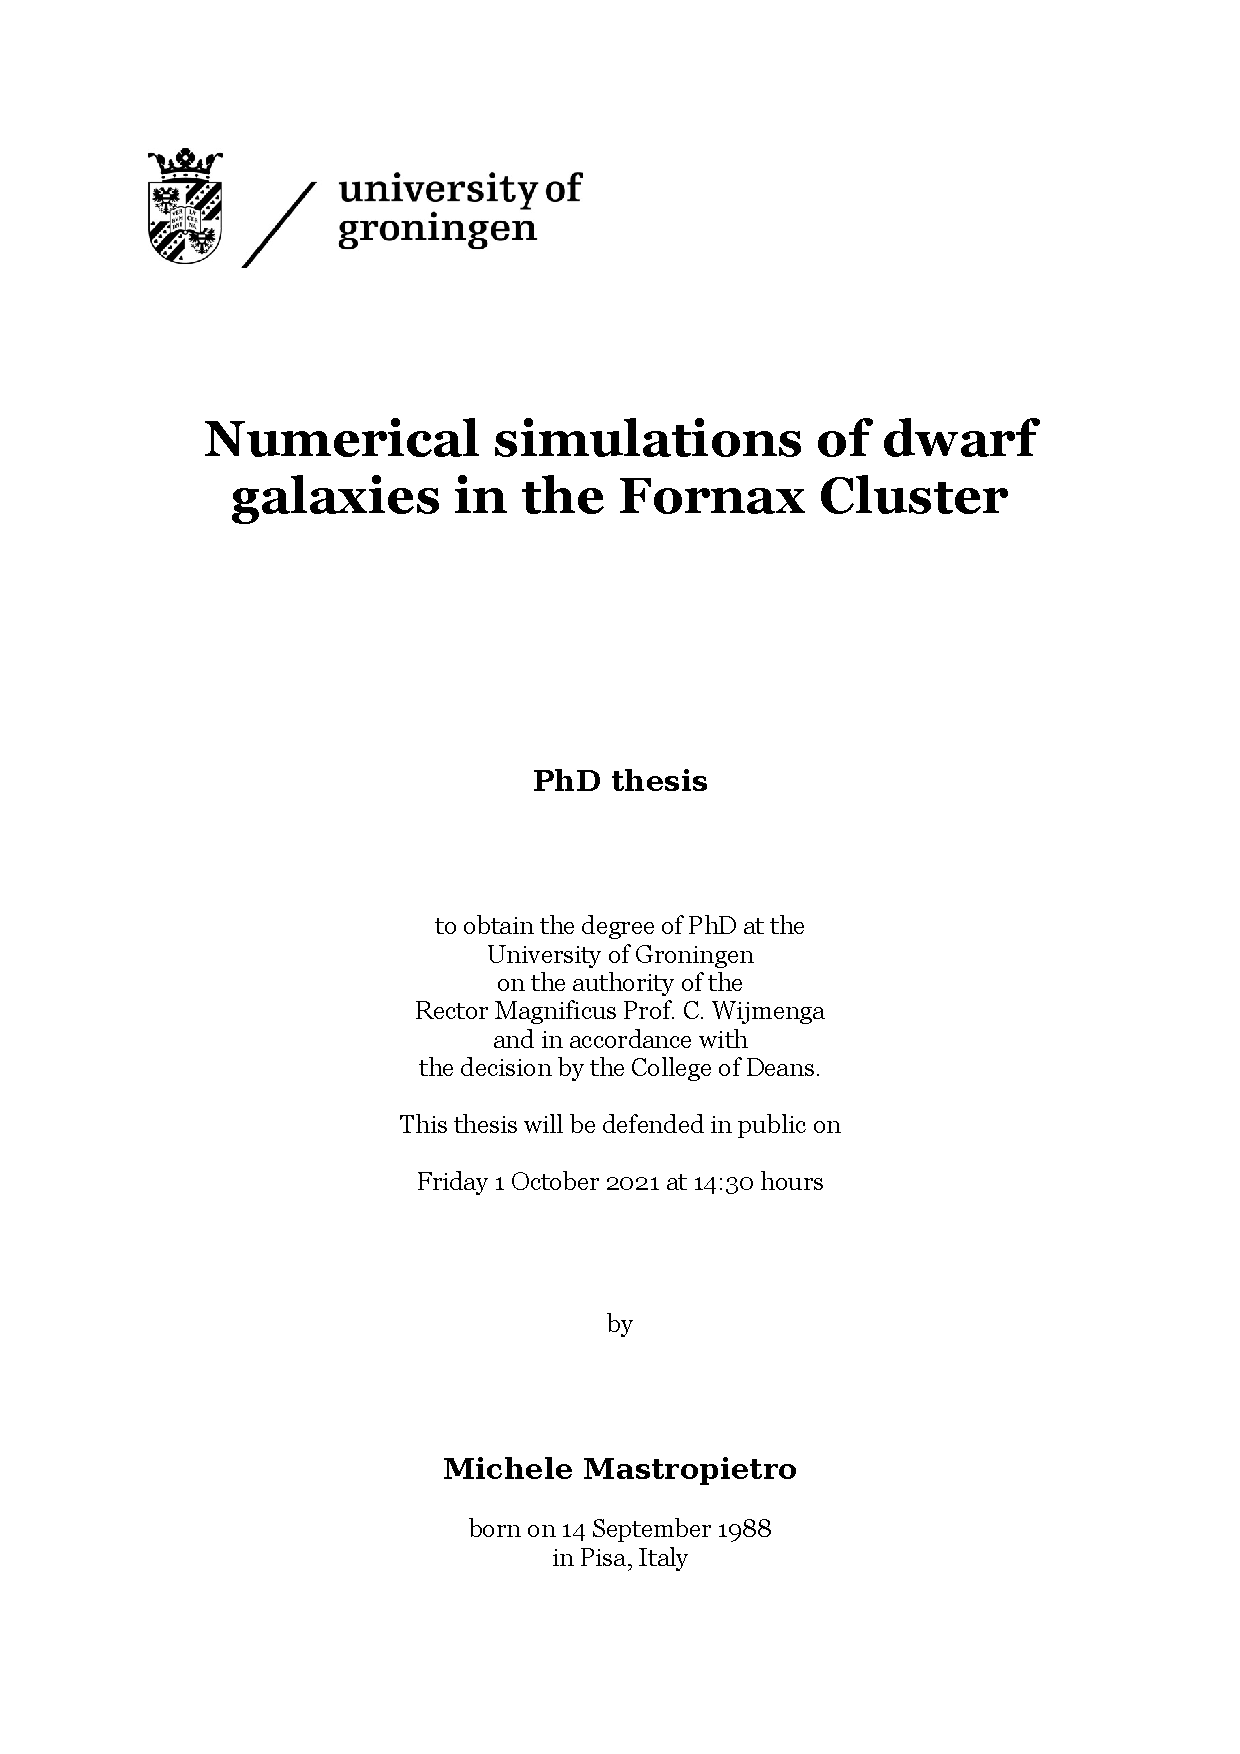
\includepdf[pages=-]{title_page.pdf}


\begin{comment}
% Official title
\begin{titlepage}
\null%
\label{thesis:title}
\vspace{3em}%
\pdfbookmark[1]{Title}{thesis:title}
\begin{center}

%% Skip space as in half-title
\vspace*{4\baselineskip}

%% Print the title.
\makeatletter
{\huge\@title}
\makeatother
\vfill

{\Large Proefschrift}

\medskip

{voorgedragen tot het behalen van \\
de graad van
Doctor in de Fysica en Sterrenkunde}


\medskip

door

\medskip

\makeatletter
{\Large \@author}
\makeatother

\medskip

aan de\\
{\large Universiteit Gent}\\
en aan de\\
{\large Rijksuniversiteit Groningen}\\
% Graduate School of Science and Engineering\\

\end{center}
\end{titlepage}





% Official verso
\clearpage
\thispagestyle{empty}
\null%
\label{thesis:committee}
\vfill
\pdfbookmark[1]{Doctoral committee}{thesis:committee}

% \noindent Members of the examination board:

\medskip\noindent
\begin{tabular}{@{}lll@{}}{Promotors:}\\\\
  \quad{}Prof.\ dr. Sven De Rijcke & Ghent University & (promotor)\\
  \quad{}Prof.\ dr. Michael\ Biehl & University of Groningen & (promotor)\\
  \quad{}Prof.\ dr. Reynier\ Peletier & University of Groningen & (promotor)\\
\\\\
\multicolumn{2}{@{}l@{}}{Composition of the Joint Evaluation Committee:} \\
\\
%   \quad{}Prof.\ dr.\  & chairperson \\
   \quad{}Prof.\ dr.\ Frazer Pearce & University of Nottingham\\
   \quad{}Prof.\ dr.\ Arjen van der Wel & Ghent University \\
   \quad{}Prof.\ dr.\ John McKean & University of Groningen \\
   \quad{}Prof.\ dr.\ Hugues Talbot & Université Paris-Saclay\\
\medskip\noindent
%   \quad{}Dr.\ & University of Groningen\\
% \\
% \multicolumn{2}{@{}l@{}}{Independent members:} \\
% \\
%   \quad{}Prof.\ dr.\ & University of Technology \\
%   \quad{}Prof.\ dr.\ & University \\
%   \quad{}Dr.\& University \\
% \\
% \multicolumn{2}{@{}l@{}}{Other member:} \\
% \\
%   \quad{}Dr.\ & ...\\
\end{tabular}
\end{comment}



% Copyright page
\clearpage
\thispagestyle{empty}
\null%
\label{thesis:colophon}
\vfill
\pdfbookmark[1]{Colophon}{thesis:colophon}
\noindent Written in 2021 by {\makeatletter{\@author}\makeatother}.\\
\textbf{Copyright}~\cczero{} The template for the layout of this thesis was inspired by my colleague Sam Verstocken who used the template of the dissertation of \href{ken.mx}{Ken Arroyo Ohori},
which was released into the public domain using the Creative~Commons~\cczero{}~code.
To view a copy of the \cczero{}~code, visit:\\\url{http://creativecommons.org/publicdomain/zero/1.0/}\\
\textbf{Colophon}
% This thesis was typeset with \XeTeX, Version 3.14159265-2.6-0.99998 (TeX Live 2017/Debian) using the \mbox{{\fanciestfont{}Feijoa}}, \texttt{GT Pressura} and $\mathrm{Asana\ Math}$ typefaces.
Most of the figures were created using \href{http://ipe.otfried.org/}{Ipe} (Copyright © 1993–2020 Otfried Cheong).
The source code of this thesis is available at: \\
\url{https://github.com/elehcim/phd-thesis}\\
\textbf{Cover}
...\\[2ex]
This research was funded by the European Union's Horizon 2020 research and innovation programme under the Marie Sk\l odowska-Curie
% Skłodowska-Curie
grant agreement N.~721463 to the \href{www.astro.rug.nl/~sundial}{SUNDIAL ITN network}.
\begin{figure*}[bh!]
  \centering
  
\includegraphics[width=0.2\textwidth]{EUflag}
\end{figure*}

% Aknowledgements page
\clearpage
\thispagestyle{empty}
\null%
\vfill
\begin{flushright}
  \textit{To my professor of physics:\\
      Mauro dell'Orso\\
      }
\end{flushright}
\vfill

% Aknowledgements page
\clearpage
\thispagestyle{empty}
\null%
\label{thesis:acknowledgements}
  \begin{center}
    {\Large \textbf{Acknowledgements}}\\
  \end{center}
\pdfbookmark[1]{Acknowledgements}{thesis:acknowledgements}
I'd like to thank first of all my professor Sven De Rijcke who believed in me doing a PhD in physics, since the first email in February 2017.
I thank you Sven for showing me what science is, how can it be beautiful and difficult and how it is a fantastic gym to train in deep honesty and integrity.
%As Feynmann said: we've learned from experience that the truth will come out, and it's this type of integrity, this kind of care not to fool yourself.
I've learned from you how to cope with work and life difficulties (especially in these pandemic times) in a very mature and ironic way.
Thank you also for being a mirror for me in our meetings, and always pushing me up even in my down moments.

The SUNDIAL project has been one of the nicest group of people I've ever met.
I'll never forget the high quality of people, their professionalism, attention and kindness for all of us. Thanks to prof. Michael Biehl, for your availability in this joint PhD journey.
Thank you prof. Reynier Peletier, our PI, practically a supervisor for all of us, always available to investigate new ideas with frank and direct attitude: %despite the many obligations and meetings you had to attend:
it's been very inspiring seeing how you live education of young scientists and astronomical research as a calling.
%Thank you Johan, my external mentor, for the interest you showed in my, for being kind and firm showing me how to clearly express.
Thanks to all of the ESRs, the one I had to work directly with: Marco, Abol, Bahar, and each one of the others: Maria Angela, Caroline, Aleke, Alex, Teymoor, Thanh, Mohammad, Shiv, Nushkia, Alan. All the best with your future.
The collaboration among us ESRs has often ended up in very good friendships, and I'll always remember the many memorable moments we lived together (in Naples, La Palma, Ghent...).

I thank my fellow astronomer colleagues at S9, the ones who are there, the ones who left during these years and the ones who just arrived.
I've learned so much from you academically and also how nice and beneficial is a happy work environment like the one you created.
The Belgian ``old guard": Maarten, Seba, Wouter, Peter, Sam, Marjorie, Dries, Robbert, Bert, Ilse, fellow Bert. Thank you for being so welcoming.
Thanks to Ana and Goran for the many moments shared together in our common expats life. Thanks to Francesco and Martina and their family: I've learned so much from you in these years we both were in Gent, much more than you think.
Caro and Pablo, thank you for all the support, deep sharing and friendship.Thank you dear office mates: Caroline, Sara, Anand and Yolan for the discussions and the nice coffee and fruit breaks.
You all have been so nice towards me, it's been an honour to work in the same place as you. Thank you for the many parties, events and dinners and many nice moments lived together.
I also thank the group of the Maxwell Demons: nice people for playing minivoetbal with fantastic team spirit.
Thank you Daniela and Andrea, young fellows of survival in lockdown times: I had so many great moments with you.
Thank you Shivangee, companion of the SUNDIAL adventure, of the office and of the life in Ghent in the happy moments as well as in the difficult times of the PhD far from home: for your constant positive attitude and for always asking how was going on for me and carefully listening. It meant a lot for me.
Thanks to Gianmarco (Jimmy), for showing me many times what true friendship means, and for being at the same time guest and host in our house in Belgium which became yours.
I thank Angelos, a real ``Sam" for me, in the sense of the Lord of the Rings: many times helping me %bringing the sometimes heavy burden of the PhD
and pulling me out of my down moments with frank conversations (is it a perk of living in Frank Baurstraat? ;P), sharing deep insights about life, cooking delicious Greek food (with an appropriate amount of garlic) and being the fuel of many parties and gatherings, with a lot of attention to everyone.

Thanks to my friends at Sint Jacobs in Gent: Davide and Ana (with the newly arrived Bea), Maria and Esteban (with the newly arrived Jose), Caique and Daniela, Valeria, Joshi, Pawel, Eligio and Luca: thank you for the improvised dinners, beers, holidays and deep friendship.
Many thanks to Pinco and the community of the Apostoline for helping me in many ways in these years: thank you for your wisdom and the constant example of free giving (gratuità).

I thank my family: mamma e babbo, for your unbreakable, positive, caring attitude towards me.
%Mi stupisco spesso di come vi siate adattati a fare i genitori di persone adulte con i fatti mostrando una strada siate davvero i genitori che vorrei avere, in tutti questi anni.
Anto for the crystalline confrontations and the enormous sensitivity, Fra for the innumerable funny stories and deep thoughts. Nonna Lida per esserci ed essere una roccia salda per tutti, always.

%Looking back at these years and looking forward for what is waiting for me,
Now that the future opens up after this beautiful adventure of the PhD, I'm on the road to find out a good way to spend my life: each of you is invaluable for orienting me in this. Thank you!

\begin{flushright}
  Gent, 14th September 2021\\Michele Mastropietro
\end{flushright}

% Summary page
\clearpage
\thispagestyle{empty}
\null%
\label{thesis:Summary}
\begin{center}
  {\Large \textbf{Summary}}\\
\end{center}
\pdfbookmark[1]{Summary}{thesis:Summary}

Dwarf galaxies are the most numerous type of stellar systems in the Universe and due to their low mass, they are very sensitive to the surrounding environment.
Because of this, they offer a privileged platform to study and isolate the different physical phenomena affecting galaxy observables.
They can be used as probes to characterize the complex interplay between internal processes and the environment in which galaxies evolve.

We carried out simulations of the evolution of dwarf galaxies falling into a Fornax-like Cluster.
We selected prototypical dwarf galaxies from the MoRIA suite of simulations and injected them one by one on different orbits.
We were interested in following the journey of the galaxies into the cluster and characterize their size, star formation rate, gas and dark matter content, stellar dynamics and evolution, depending on the orbit and the initial mass at the time of orbital injection.
To do so, we implemented the Moving Box simulation technique in our in-house simulation code.
This allows us to simulate the dwarf-cluster interaction at high resolution while keeping an affordable run time.

We found that during infall, generally, galaxies undergo some ``phase transitions" which happen mainly at pericenter passages.
Some of the galaxies are effectively transformed into Ultra Diffuse Galaxies (UDG) while some others are allowed to be briefly identified as ``jellyfish".
It is therefore possible to hypothesize that the jellyfish phenomenon is a relatively short transitory phase of a dwarf galaxy along its orbit, and it's likely a precursor of the transformation of a dwarf galaxy into an UDG.

Serendipitously we realized that our simulations produce galaxies whose morphology is similar to a galaxy in the Fornax Cluster with a peculiar  \Hi{} tail and an arrow-shaped stellar body oriented in different directions: NGC~1427A.
Multiple formation scenarios have been proposed for this galaxy, but a consensus was still lacking in the literature.
We identified that gaseous and stellar tails pointing in different directions are explainable given that they are subject to different environmental effects (ram-pressure stripping and tidal forces). This idea finds support in our simulations and we developed a procedure to quantitatively assess the properties of simulated galaxies from a catalogue of simulations.
We were also able to provide some falsifiable predictions on the position of the galaxy with respect to the center of the Cluster and its projected orbital direction.

Finally, we contributed to the development of a technique to study low dimensional-manifolds in the simulations.
We found that the technique can be very useful to isolate the physical properties of filaments in N-body simulations.
In particular we concentrated on the analysis of gaseous tails of simulated Jellyfish galaxies with the aim to investigate regions of recent star formation and mixing between the galactic gaseous material and the hot gas of the cluster.


\clearpage
\thispagestyle{empty}
\null%
\begin{center}
  {\Large \textbf{Samenvatting}}\\
\end{center}

%\begin{otherlanguage*}{dutch}
Dwerggalaxieën zijn het talrijkste type sterrenstelsels in het heelal en door hun lage massa zijn zij zeer gevoelig voor hun omgeving.
Daarom bieden zij een bevoorrecht platform om de verschillende fysische fenomenen die de waarneembare eigenschappen van sterrenstelsels beïnvloeden, te bestuderen en te isoleren.
Ze kunnen worden gebruikt als laboratoria om de complexe wisselwerking tussen interne processen en de omgeving waarin galaxieën evolueren te onderzoeken en te karakteriseren.

Wij hebben simulaties uitgevoerd van de evolutie van verschillende dwerggalaxieën die in een Fornax-achtige Cluster vallen.
We selecteerden prototypische dwerggalaxieën uit de MoRIA-simulatiesuite en injecteerden ze één voor één op verschillende banen.
We waren geïnteresseerd in het volgen van de reis van de melkwegstelsels in de cluster en het karakteriseren van hun grootte, stervormingssnelheden, hun inhoud aan gas en donkere materie, hun interne dynamica en hun evolutie, afhankelijk van de baan en de initiële massa op het moment van de injectie in de baan.
Daartoe hebben wij de Moving-Box-simulatietechniek aangepast aan onze noden en geïmplementeerd in onze eigen simulatiecode.
Dit maakt het mogelijk om de dwerg-clusterinteractie met zeer hoge resolutie te simuleren binnen een haalbare totale runtijd.

We ontdekten dat tijdens de inval, over het algemeen, melkwegstelsels enkele faseovergangen ondergaan, die voornamelijk  plaatsvinden bij pericenterpassages.
Sommige van de stelsels  worden getransformeerd in Ultra Diffuse Galaxies (UDG), andere worden kortstondig geïdentificeerd als ``jellyfish''.
Het is daarom mogelijk te veronderstellen dat het ``jellyfish"-fenomeen een relatief korte overgangsfase is van een dwergmelkwegstelsel langs zijn baan, en waarschijnlijk een voorloper is van de transformatie van een dwerggalaxie in een UDG.

Dankzij enige serendipiteit realiseerden we ons dat onze simulaties melkwegstelsels produceren waarvan de morfologie vergelijkbaar is met die van een welbepaald melkwegstelsel in de Fornax Cluster met een eigenaardige  \Hi{} staart en een pijlvormig stellair lichaam die in verschillende richtingen georiënteerd zijn: NGC~1427A.
Voor dit sterrenstelsel zijn meerdere formatiescenario's voorgesteld, maar in de literatuur was er nog geen consensus over.
Wij stelden vast dat gasvormige en stellaire staarten die in verschillende richtingen wijzen verklaarbaar zijn, aangezien zij onderhevig zijn aan verschillende omgevingseffecten (ramdruk en getijdekrachten).
Dit wordt ondersteund door onze simulaties en wij hebben een procedure ontwikkeld om de eigenschappen van gesimuleerde melkwegstelsels kwantitatief te beoordelen aan de hand van een catalogus van simulaties.
We waren ook in staat om enkele falsifieerbare voorspellingen te doen over de positie van het melkwegstelsel ten opzichte van het centrum van de Cluster en zijn geprojecteerde baanrichting.

Tenslotte hebben we bijgedragen aan de ontwikkeling van een techniek om laagdimensionale manifolds in simulaties de bestuderen.
We ontdekten dat de techniek zeer nuttig kan zijn om de fysische eigenschappen van filamenten in N-body-simulaties te isoleren.
In het bijzonder hebben we ons geconcentreerd op de analyse van gasvormige staarten van gesimuleerde ``jellyfish"-sterrenstelsels met het doel regio's van recente stervorming en vermenging tussen het galactische gasachtige materiaal en het hete gas van de cluster te onderzoeken.
%\end{otherlanguage*}

\clearpage
\thispagestyle{empty}
\null%
\begin{center}
  {\Large \textbf{Riassunto}}\\
\end{center}
\begin{otherlanguage*}{italian}
Le galassie nane sono i sistemi stellari più numerosi dell'Universo e, a causa della loro piccola massa, sono molto sensibili all'ambiente che sta loro intorno.
Per questo motivo, offrono una piattaforma privilegiata per studiare e isolare i diversi fenomeni fisici che influenzano le caratteristiche osservabili delle galassie.
Possono essere utilizzati come sonde per caratterizzare la complessa interazione tra i processi interni e l'ambiente in cui le galassie si evolvono.

Abbiamo effettuato simulazioni dell'evoluzione delle galassie nane che cadono in un ammasso con caratteristiche simili a quello della Fornace.
Con alcune galassie prototipali selezionate dalla suite di simulazioni MoRIA e abbiamo messe su una per una su diverse orbite.
È di interesse scientifico seguire il viaggio delle galassie nell'ammasso e a caratterizzare le loro dimensioni, la formazione stellare, il contenuto di gas e materia oscura, la dinamica stellare e la sua evoluzione, a seconda dell'orbita e della massa iniziale al momento dell'iniezione orbitale.
Per fare ciò, abbiamo implementato la tecnica di simulazione chiamata ``Moving Box" nel codice sviluppato nel nostro dipartimento.
Questo ci ha permetto di simulare l'interazione galassia nana ammasso ad alta risoluzione mantenendo un pratico tempo di calcolo.

Abbiamo trovato che durante l'orbita, generalmente, le galassie subiscono alcune ``transizioni di fase" che avvengono principalmente attorno al passaggio per il pericentro.
Alcune galassie vengono effettivamente trasformate in Galassie Ultra Diffuse (UDG), mentre altre possono essere identificate brevemente come ``galassie medusa'' (jellifish).
È quindi possibile ipotizzare che il fenomeno delle galassie medusa sia una fase transitoria relativamente breve di una galassia nana lungo la sua orbita, e che constituisca probabilmente un precursore della trasformazione di una galassia nana in una UDG.

Per una fortuita combinazione, abbiamo notato che le nostre simulazioni producono galassie la cui morfologia è simile a quella di una galassia dell'ammasso della Fornace con una peculiare coda \Hi{} e un corpo stellare a forma di freccia, orientate in diverse direzioni: la NGC~1427A.
Per questa galassia sono stati proposti molteplici scenari di formazione, ma manca ancora un consenso in letteratura.
Abbiamo identificato che le code gassose e stellari che puntano in direzioni diverse sono spiegabili dato che ognuna è soggetta a diversi effetti ambientali (pressione e forze di marea).
Questa idea trova supporto nelle nostre simulazioni.
Abbiamo quindi sviluppato una procedura per valutare quantitativamente le proprietà delle galassie simulate partendo da un catalogo di simulazioni.
Siamo stati anche in grado di fornire alcune previsioni falsificabili sulla posizione della galassia rispetto al centro dell'ammasso e la sua direzione orbitale proiettata.

Infine, abbiamo contribuito allo sviluppo di una tecnica per studiare nelle simulazioni le varietà (manifold) con una dimensionalità bassa.
Abbiamo scoperto che questa tecnica può essere molto utile per isolare le proprietà fisiche dei filamenti nelle simulazioni N corpi.
In particolare, ci siamo concentrati sull'analisi delle code gassose delle galassie medusa simulate con l'obiettivo di indagare le regioni di recente formazione stellare e di mescolamento tra il materiale gassoso galattico e il gas caldo dell'ammasso.
\end{otherlanguage*}